\chapter{Christ Defeats Satan (20:1--20:15)}\index{Satan}

The twentieth chapter brings us at last before the great white throne\index{great white throne}. On that day, every person will stand before God. No one, great or small, will escape the final judgment\index{judgment}, regardless of the power, wealth, or renown they possessed in this world. Neither death nor Hades\index{Hades} can offer a permanent refuge. The books will be opened, and every life will be laid bare before God.

This chapter has also been interpreted in different ways. Is the thousand years a literal period of a thousand years, or does it symbolize a complete span of time? Does the ``first resurrection\index{first resurrection}'' refer to the resurrection of the body or to spiritual life? Will Christ reign on earth for a thousand years, or is He already reigning? What does it mean for Satan\index{Satan} to be bound? Generations of Christians have wrestled seriously with these questions, giving rise to different positions on the end times\index{end times}.

Yet as we read this chapter, we must not allow these questions to obscure what John most wants us to see. Satan\index{Satan} is not the final King. Christ is. And the question we must ask ourselves is this: ``Since Christ will surely triumph, how should I faithfully follow Him today?''

\section{Satan Bound, the Saints Reigning with Christ}\index{Satan}

\begin{figure}[htbp]
    \centering
    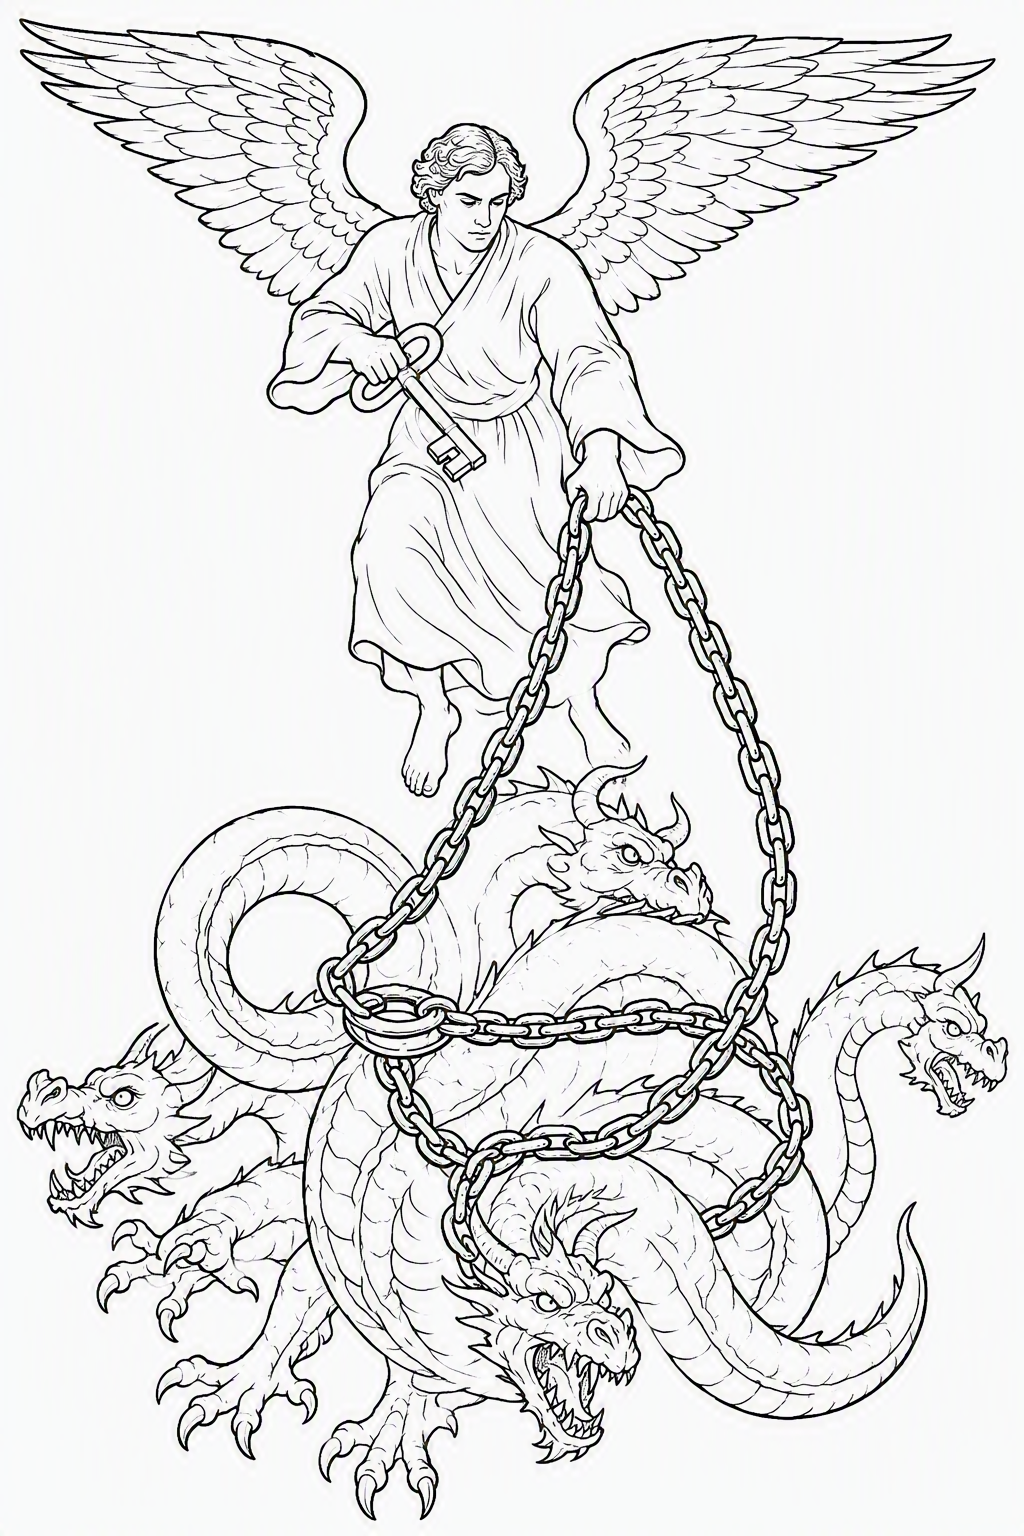
\includegraphics[
    width=0.6\textwidth,
    trim=0 0 0 0,
    clip]{images/rev20-satan-bound.png}
\end{figure}

\begin{ScriptureBox}

\item[20:1] And I saw an angel coming down out of heaven, having the key to the Abyss and holding in his hand a great chain.

\item[20:2] He seized the dragon, that ancient serpent, who is the devil, or Satan, and bound him for a thousand years.

\item[20:3] He threw him into the Abyss, and locked and sealed it over him, to keep him from deceiving the nations anymore until the thousand years were ended. After that, he must be set free for a short time.

\item[20:4] I saw thrones on which were seated those who had been given authority to judge. And I saw the souls of those who had been beheaded because of their testimony about Jesus and because of the word of God. They had not worshiped the beast or its image and had not received its mark on their foreheads or their hands. They came to life and reigned with Christ a thousand years.
% NIV footnote for 20:4 (omitted; add as \footnote if wanted):
%   ``They'' --- Or God; I also saw those who
% CHECK NIV: footnote wording quoted from memory; verify against Bible Gateway.

\item[20:5] (The rest of the dead did not come to life until the thousand years were ended.) This is the first resurrection.

\item[20:6] Blessed and holy are those who share in the first resurrection. The second death has no power over them, but they will be priests of God and of Christ and will reign with him for a thousand years.

\item[20:7] When the thousand years are over, Satan will be released from his prison

\end{ScriptureBox}

From these verses, we learn that Satan\index{Satan}, though still a real adversary, is subject to God's authority and restraint. Those who remain faithful to Christ will share in His reign.

But perhaps you find yourself asking, ``Why does God not destroy Satan\index{Satan} immediately? Why bind him first, rather than bring his existence to an end?''

This is no minor question. Christians have considered it for centuries, from the age of the early Church Fathers to the present day. It is worth taking a moment to understand how different generations have approached it.

\subsection{Why Not Destroy Satan Immediately?}\index{Satan}

Early Church Fathers such as Justin Martyr\index{martyrs} and Irenaeus\index{Irenaeus} generally understood Satan\index{Satan}'s binding as a future event. After a period of great tribulation\index{Great Tribulation}, Christ would return, bind Satan, and reign on earth for a thousand years. This interpretation became known as premillennialism\index{premillennialism}. The prefix ``pre-'' indicates that Christ's return precedes the millennium\index{millennium}.

A significant change in interpretation came with Augustine. In his work \textit{The City of God}, he argued that Satan\index{Satan} was already bound. The thousand years represented the age of the Church, extending from Christ's first coming to the end of the present age. This binding did not mean that Satan was entirely inactive. Rather, God had restrained his power to deceive the nations, allowing the gospel to go forth among the peoples of the world.

Western Christianity during the Middle Ages largely followed Augustine's understanding. Satan\index{Satan} could still tempt and attack humanity, but his power was limited by God's sovereign purpose. At the end of the age, he would face his final judgment. This interpretation became known as amillennialism\index{amillennialism}.

In more recent centuries, premillennial\index{premillennialism} interpretations have also received considerable attention, with different forms of premillennialism developing within the broader Christian tradition.

\subsection{Who Are the Inhabitants of the Earth?}

If the resurrected saints reign with Christ, we may naturally ask: Who inhabits the earth during the millennium\index{millennium}?

In the premillennial\index{premillennialism} interpretation presented here, two groups of people may be distinguished:

\begin{itemize}
    \item \textbf{The resurrected saints:} They possess glorified\index{glory}, imperishable bodies and reign with Christ.
    \item \textbf{The mortal inhabitants:} They continue to live in mortal bodies under Christ's righteous rule and have descendants.
\end{itemize}

This distinction belongs to a particular understanding of the millennium\index{millennium}. Other interpretations understand the thousand years differently and do not necessarily envision two such groups living on earth during that period.

\subsection{The Millennium}\index{millennium}

Christians have traditionally discussed three major positions concerning the millennium\index{millennium}: premillennialism\index{premillennialism}, postmillennialism\index{postmillennialism}, and amillennialism\index{amillennialism}. A comparison of these views appears in the appendix, ``Millennial Views.''

Here, we will first consider the premillennial\index{premillennialism} interpretation. According to this view, Christ will return personally before the millennium\index{millennium}, bind Satan\index{Satan}, raise the martyred\index{martyrs} saints, and reign with them on earth for a thousand years. At the end of this period, Satan will be released and instigate one final rebellion. His revolt will be crushed, and he will be cast into the lake of fire\index{lake of fire} forever.

Whether one holds to premillennialism\index{premillennialism}, postmillennialism\index{postmillennialism}, or amillennialism\index{amillennialism}, the ultimate message of Revelation 20 remains clear: Satan\index{Satan} will be defeated, and Christ's kingdom will reach its consummation in glory.

\section{The Final Battle: Gog and Magog}\index{Gog and Magog}

\begin{figure}[htbp]
    \centering
    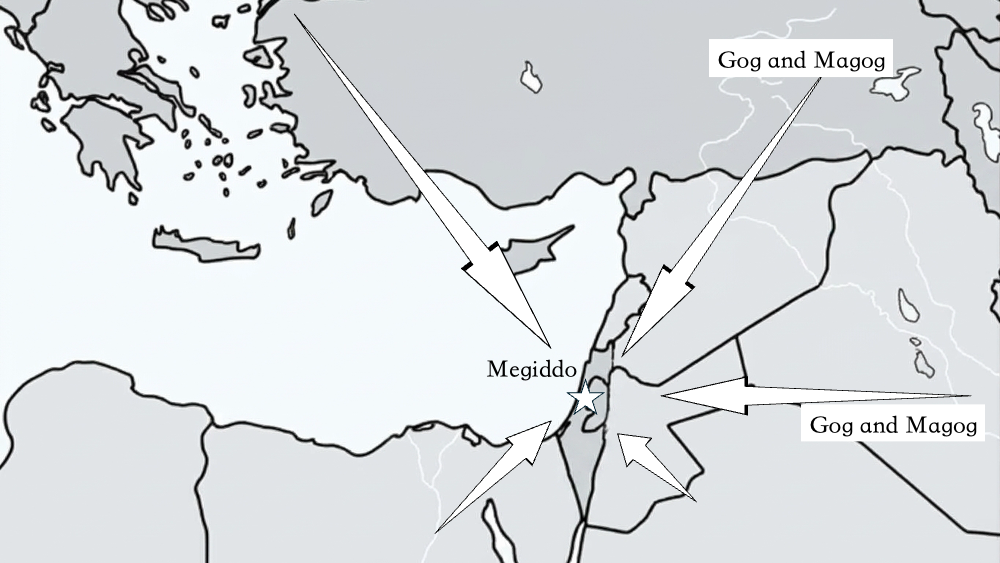
\includegraphics[
    width=1\textwidth,
    trim=0 0 0 0,
    clip]{images/Armageddon_english.png}
\end{figure}

\begin{ScriptureBox}

\item[20:8] and will go out to deceive the nations in the four corners of the earth---Gog and Magog---and to gather them for battle. In number they are like the sand on the seashore.

\item[20:9] They marched across the breadth of the earth and surrounded the camp of God's people, the city he loves. But fire came down from heaven and devoured them.

\item[20:10] And the devil, who deceived them, was thrown into the lake of burning sulfur, where the beast and the false prophet had been thrown. They will be tormented day and night for ever and ever.

\end{ScriptureBox}

Although Gog and Magog\index{Gog and Magog} appear in only one verse of Revelation 20, these names have a much longer history in biblical prophecy. They already appear in Ezekiel\index{Ezekiel} 38--39, where Gog comes from the far north and leads a great coalition of nations against God's people.

In Revelation, however, Gog and Magog\index{Gog and Magog} are portrayed as nations gathered from the four corners of the earth. They surround the camp of the saints and the beloved city, only to be consumed when fire comes down from heaven (Revelation 20:9).

John is drawing upon Ezekiel's prophetic imagery, but he presents it from a somewhat different perspective. This may be described as an eschatological reconfiguration: Revelation does not merely repeat the Old Testament's visions of the end. It brings together familiar prophetic images and places them within the unfolding story of Christ's redemption\index{redemption} and God's final judgment, allowing those images to serve a renewed purpose.

One detail is especially worth noting. In Revelation 19, Christ defeats the hostile forces gathered for the battle associated with Armageddon\index{Armageddon}. In Revelation 20, the vision of Gog and Magog\index{Gog and Magog} portrays the destruction of the forces of evil once more, now from a different angle.

Christians differ over whether these visions describe distinct events in chronological succession or portray the same ultimate conflict from different perspectives. Yet both visions declare the same truth: evil may gather its forces in a final, desperate rebellion, but its defeat is certain.

The nations may rise in overwhelming numbers. Their armies may surround the beloved city. For a moment, their power may seem irresistible. Yet the outcome does not depend on the strength of God's people or the size of their enemies. The final word belongs to God. The fire descends from heaven, the rebellion ends, and Satan\index{Satan}'s power is brought to its everlasting judgment.

\section{The Final Judgment: Before the Great White Throne}\index{great white throne}\index{judgment}

\begin{ScriptureBox}

\item[20:11] Then I saw a great white throne and him who was seated on it. The earth and the heavens fled from his presence, and there was no place for them.

\item[20:12] And I saw the dead, great and small, standing before the throne, and books were opened. Another book was opened, which is the book of life. The dead were judged according to what they had done as recorded in the books.

\item[20:13] The sea gave up the dead that were in it, and death and Hades gave up the dead that were in them, and each person was judged according to what they had done.

\item[20:14] Then death and Hades were thrown into the lake of fire. The lake of fire is the second death.

\item[20:15] Anyone whose name was not found written in the book of life was thrown into the lake of fire.

\end{ScriptureBox}

John now sees a great white throne\index{great white throne}. Before the One seated upon it, heaven and earth flee away, and no place remains for them. The present order of creation is passing away, and God's final judgment has arrived.

The dead stand before the throne\index{throne of God}, great and small alike. The books are opened, and another book is opened as well: the book of life\index{book of life}. All are judged according to what is recorded in the books, according to what they have done.

No one can evade this final reckoning. No earthly distinction can shield anyone from the gaze of the One who judges. Rank and reputation, wealth and poverty, greatness and obscurity—all fall away before the throne of God. Every life must answer to Him.

The vision is solemn, and we should not soften its warning. Yet it also brings the whole story of Revelation into sharp focus. The evil that once seemed unconquerable has been overthrown. Satan\index{Satan} has been cast into the lake of fire\index{lake of fire}. Even Death and Hades\index{Hades} are abolished. The enemies that have tormented God's creation will not endure forever.

The final division is absolute: life or the second death\index{second death}. Those whose names are written in the book of life\index{book of life} belong to God; those whose names are not found there face the judgment of the lake of fire\index{lake of fire}.

This vision calls us to examine our lives honestly, but it also directs our attention beyond our own deeds to the God before whom every person must stand. The book of life\index{book of life} reminds us that our ultimate hope cannot rest in worldly achievement or self-assurance. It rests in God's saving grace\index{grace} and in the victory of Jesus Christ, the Lamb who was slain\index{Lamb, the!slain} and who reigns forever.

\begin{figure}[htbp]
    \centering
    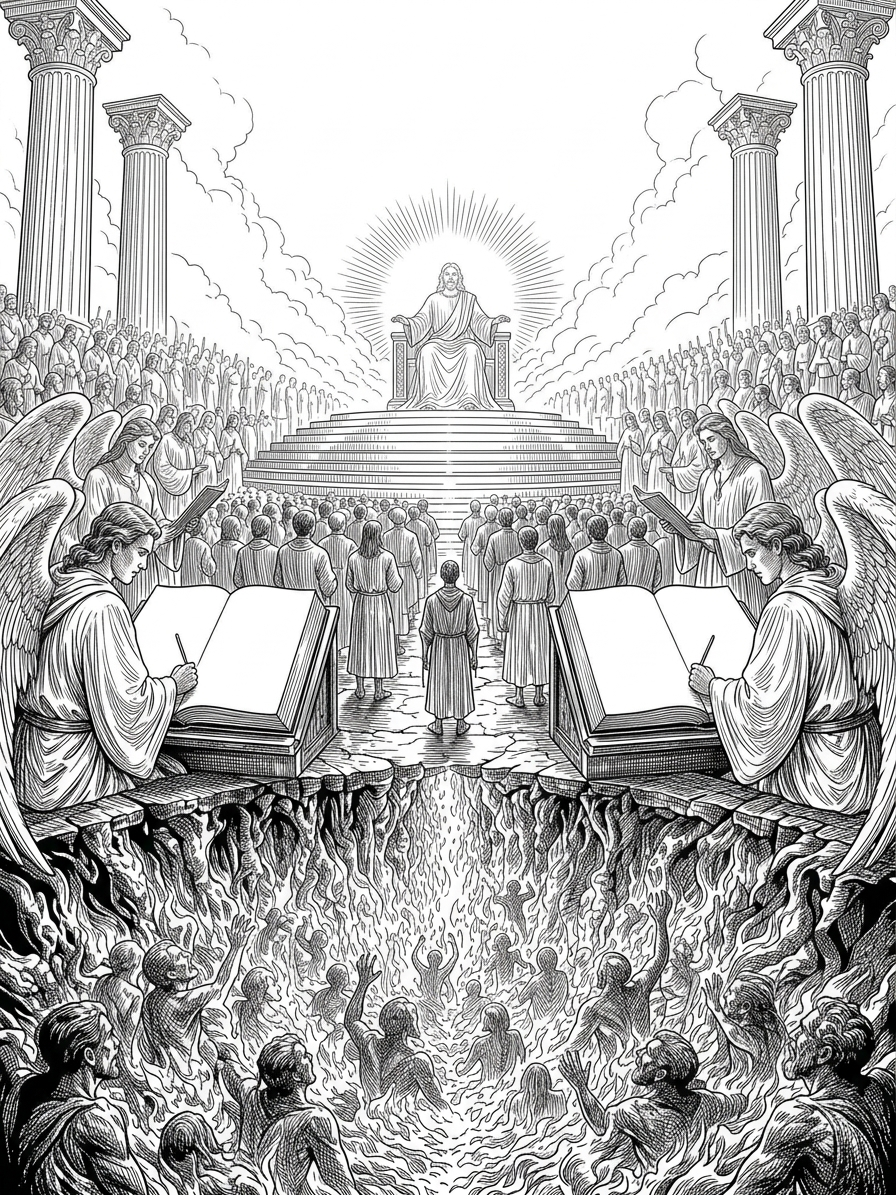
\includegraphics[
    width=1\textwidth,
    trim=0 0 0 0,
    clip]{images/white_throne_judgement.jpg}
\end{figure}

\section*{Discussion Questions}

\begin{enumerate}

    \item Read Revelation 20:11--15, the vision of the great white throne. What is your strongest response to this passage: a sense of warning, reverence, comfort, or hope? Why?

    \item If you are confident that Christ will ultimately triumph, that Satan will be defeated, and that death itself will be abolished, how might this confidence change the way you live today? In your family, at work, in the church, or amid suffering, what truth do you most need to hold fast to?

\end{enumerate}